%!TEX root = ../main.tex

\section{Experiment 1: FOCUS vs. FT}
\label{section:experiment1}



We compare FOCUS to the Feature Tweaking (FT) method by \citet{tolomei_interpretable_2017} in terms of the evaluation metrics in Section~\ref{section:focus-evalmetrics}. 
We consider \numprint{36} experimental settings (\numprint{4} datasets $\times$ \numprint{3} tree-based models $\times$ \numprint{3} distance functions) when comparing FOCUS to FT. 
The results are listed in Table~\ref{table:distances}. 

\subsection{Baseline: Feature Tweaking}
\label{section:baselineft}
FT identifies the leaf nodes where the prediction of the leaf nodes do not match the original prediction $y_x$: it recognizes the set of leaves that if activated, $t_j(\bar{x}) = 1$, would change the prediction of a tree $\mathcal{T}$:
\begin{equation}
\mathcal{T}_\textit{change} = \left\{ j \mid j \in   \mathcal{T}_\textit{leaf} \land y_x \not = \arg \max_y T(y\mid j) \right\}.
\end{equation}
For every $\mathcal{T}$ in $f$, FT generates a perturbed example per node in $\mathcal{T}_\textit{change}$ so that it is activated with at least an $\epsilon$ difference per threshold, and then selects the most optimal example (i.e., the one closest to the original instance).
For every feature threshold $\theta_j$ involved, the corresponding feature is perturbed accordingly: $\bar{x}_{f_j} = \theta_j \pm \epsilon$.
The result is a perturbed example that was changed minimally to activate a leaf node in $\mathcal{T}_\textit{change}$. 
In our experiments, we test $\epsilon \in \{0.001, 0.005, 0.01, 0.1\}$, and choose the $\epsilon$ that minimizes the mean distance to the original input, while maximizing the number of counterfactual examples generated. 


The main problem with FT is that the perturbed examples are not necessarily counterfactual examples, since changing the prediction of a single tree $\mathcal{T}$ does not guarantee a change in the prediction of the full ensemble $f$.
Figure~\ref{fig:approxensemble} shows all three perturbed examples generated by FT for a single instance. 
In this case, none of the generated examples change the model prediction and therefore none are valid counterfactual examples. 

Figure~\ref{fig:approxensemble} shows how FOCUS and FT handle an adaptive boosting ensemble using a two-feature ensemble with three trees. 
On the left is the decision boundary for a standard tree ensemble; the middle visualizes the positive leaf nodes that form the decision boundary; on the right is the approximated loss $\widetilde{\mathcal{L}}_{pred}$ and its gradient w.r.t. $\bar{x}$.
The gradients push features close to thresholds harder and in the direction of the decision boundary if $\widetilde{\mathcal{L}}$ is convex. 


\subsection{Results}
In terms of $d_\mathit{mean}$, FOCUS outperforms FT in \numprint{20} settings while FT outperforms FOCUS in \numprint{8} settings. The difference in $d_\mathit{mean}$ is not significant in the remaining \numprint{8} settings. 
In general, FOCUS outperforms FT in settings using Euclidean and Cosine distance because in each iteration, FOCUS perturbs many of the features by a small amount. 
Since FT perturbs only the features associated with an individual leaf, we expected that it would perform better for Manhattan distance but our results show that this is not the case. 
There is no clear winner between FT and FOCUS for Manhattan distance. 

\begin{figure}[t]
\centering

\includegraphics[scale=0.23]{04-research-focus/figures/decision_example} 
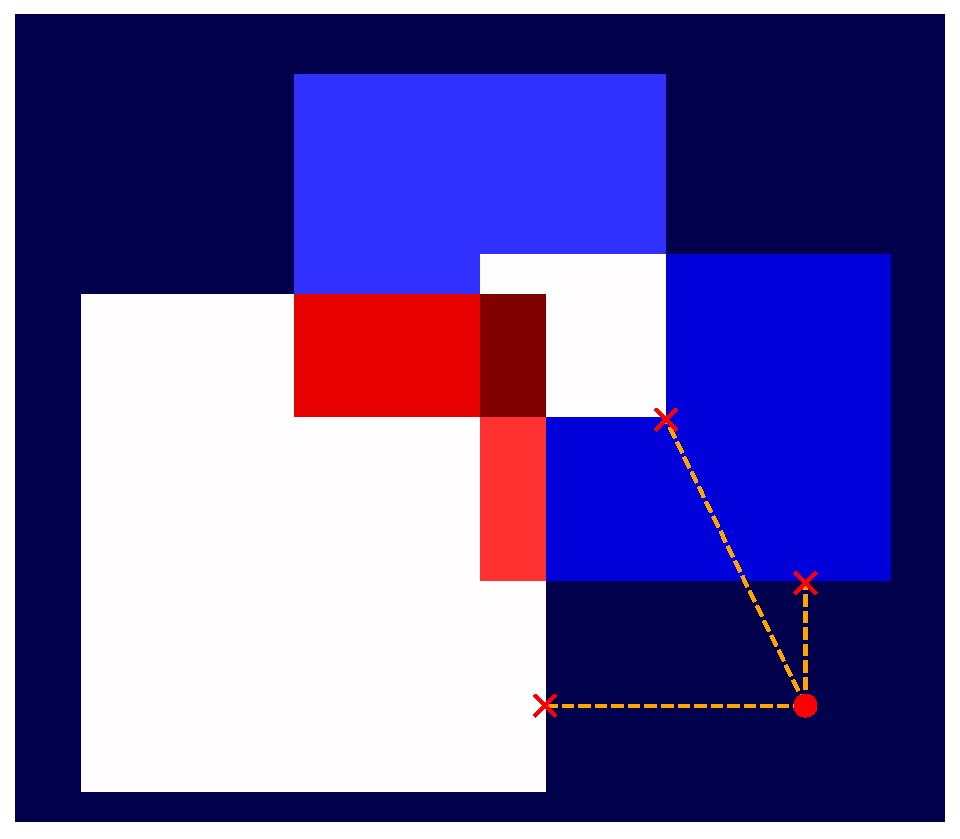
\includegraphics[scale=0.23]{04-research-focus/figures/leaf_example} 
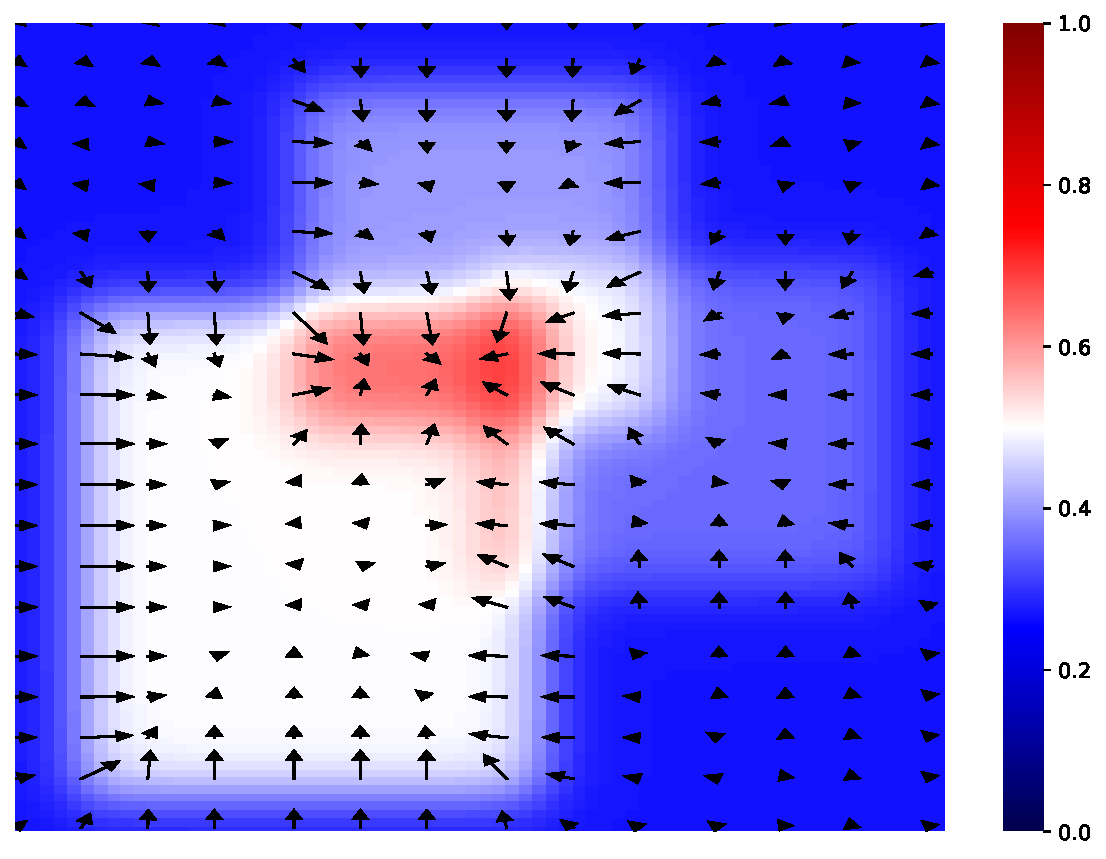
\includegraphics[scale=0.23]{04-research-focus/figures/approx_example}
\caption{
An example of how the FT baseline method (explained in Section~\ref{section:baselineft}) and our method handle an adaptive boosting ensemble with three trees.
Left: decision boundary of the ensemble.
Middle: three positive leaves that form the decision boundary, an example instance, and the perturbed examples suggested by \acs{FT}. 
Right: approximated loss $\widetilde{\mathcal{L}}_{pred}$ and its gradient w.r.t. $\bar{x}$. 
The \acs{FT} perturbed examples do not change the prediction of the forest, whereas the gradient of the differentiable approximation leads toward the true decision boundary.
}
\label{fig:approxensemble}
\end{figure}



\begin{landscape}
\begin{table}
\caption{Evaluation results for Experiment 1 comparing FOCUS and FT counterfactual examples. Significant improvements and losses over the baseline (FT) are denoted by \dubbelneer\ and \dubbelop, respectively ($p < 0.05$, two-tailed t-test,); 
\notsig{} denotes no significant difference;
\NoExample{} denotes settings where the baseline cannot find a counterfactual example for every instance.}
%!TEX root = ../main.tex

\begin{tabular}{llrrrrrrrrrr}
\toprule
  &                   &                  & \multicolumn{3}{c}{\textbf{Euclidean}}                                                              & \multicolumn{3}{c}{\textbf{Cosine}}                                                                 & \multicolumn{3}{c}{\textbf{Manhattan}}                                                              \\
  \cmidrule(r){4-6}\cmidrule(r){7-9} \cmidrule(r){10-12}
 \textbf{Dataset}                 &     \textbf{Metric}                & \textbf{Method}                 & \multicolumn{1}{c}{\textbf{DT}} & \multicolumn{1}{c}{\textbf{RF}} & \multicolumn{1}{c}{\textbf{AB}} & \multicolumn{1}{c}{\textbf{DT}} & \multicolumn{1}{c}{\textbf{RF}} & \multicolumn{1}{c}{\textbf{AB}} & \multicolumn{1}{c}{\textbf{DT}} & \multicolumn{1}{c}{\textbf{RF}} & \multicolumn{1}{c}{\textbf{AB}} \\
 \midrule
\textit{}        &    $d_{mean}$                & FT               & 0.269 & \textbf{0.174}  & 0.267\rlap\NoExample  & 0.030 & 0.017  & 0.034\rlap\NoExample  & 0.269 & \textbf{0.223} & 0.382\rlap\NoExample  \\
\textsc{Wine}    &                    & FOCUS              & \textbf{0.268}\rlap{\notsig} & 0.188\rlap{\dubbelop}   & \textbf{0.188}\rlap{\dubbelneer}  & \textbf{0.003}\rlap{\dubbelneer} & \textbf{0.008}\rlap{\dubbelneer}  & \textbf{0.014}\rlap{\dubbelneer}  & \textbf{0.268}\rlap{\notsig} & 0.312\rlap{\dubbelop} & \textbf{0.360}\rlap{\dubbelneer}  \\
\cmidrule{2-12}
\textsc{Quality}        &       $d_{Rmean}$             & FOCUS/FT           & 0.990 & 1.256  & 0.649  & 0.066 & 0.821  & 0.312  & 0.990 & 1.977 & 0.924  \\
%\cmidrule{2-12}
\textit{}        &      $\mathit{\%_{closer}}$              & FOCUS \textless FT                           & 100\% & 21.0\% & 87.5\% & 100\% & 80.8\% & 95.1\% & 100\% & 5.4\% & 58.6\%                           \\





\midrule


                 &      $d_{mean}$              & FT               & \textbf{0.120}  & 0.210  & 0.185  & 0.003  & 0.008  & 0.007  & \textbf{0.135}  & \textbf{0.278}  & \textbf{0.198}  \\
  \textsc{HELOC}               &                    & FOCUS              & 0.133\rlap{\dubbelop}  & \textbf{0.186}\rlap{\dubbelneer}  & \textbf{0.136}\rlap{\dubbelneer}  & \textbf{0.001}\rlap{\dubbelneer}  & \textbf{0.002}\rlap{\dubbelneer}  & \textbf{0.001}\rlap{\dubbelneer}  & 0.152\rlap{\dubbelop}  & 0.284\rlap{\notsig}  & 0.203\rlap{\notsig}  \\
\cmidrule{2-12}

                 &     $d_{Rmean}$               & FOCUS/FT           & 1.169  & 0.942  & 0.907  & 0.303  & 0.285  & 0.421  & 1.252  & 1.144  & 1.364  \\ 
%\cmidrule{2-12}
                 &     $\mathit{\%_{closer}}$               & FOCUS \textless FT & 16.6\% & 57.9\% & 71.9\% & 91.6\% & 91.5\% & 92.9\% & 51.3\% & 43.6\% & 24.2\%          \\
 
 \midrule
 
 
 
 

                 &      	$d_{mean}$              & FT               & \textbf{0.082} & \textbf{0.075} & 0.081 & 0.013 & 0.014 & 0.015 & \textbf{0.086} & \textbf{0.078} & \textbf{0.085} \\
  \textsc{COMPAS}               &              & FOCUS              & 0.092\rlap{\dubbelop} & 0.079\rlap{\notsig} & \textbf{0.076}\rlap{\dubbelneer} & \textbf{0.008}\rlap{\dubbelneer} & \textbf{0.011}\rlap{\dubbelneer} & \textbf{0.007}\rlap{\dubbelneer} & 0.093\rlap{\dubbelop} & 0.085\rlap{\notsig} & 0.090\rlap{\notsig} \\
\cmidrule{2-12}
                 &      $d_{Rmean}$              & FOCUS/FT           & 1.162 & 1.150 & 1.062 & 0.473 & 0.965 & 0.539 & 1.182 & 1.236 & 1.155 \\ 
%\cmidrule{2-12}
                 &      $\mathit{\%_{closer}}$              & FOCUS \textless FT & 29.4\% & 22.6\% & 44.8\% & 82.7\% & 68.0\% & 84.8\% & 65.8\% & 36.2\% & 66.9\% \\
\midrule






                 &      	$d_{mean}$              & FT                & \textbf{0.119}  & 0.028  & 0.126\rlap\NoExample  & \textbf{0.050}  & 0.027  & 0.131\rlap\NoExample  & \textbf{0.121}  & 0.030  & 0.142\rlap\NoExample  \\
   \textsc{Shopping}              &              & FOCUS              & 0.142\rlap{\dubbelop}  & \textbf{0.025}\rlap{\dubbelneer}  & \textbf{0.028}\rlap{\dubbelneer}  & 0.055\rlap{\dubbelop}  & \textbf{0.013}\rlap{\dubbelneer}  & \textbf{0.006}\rlap{\dubbelneer}  & 0.128\rlap{\notsig}  & \textbf{0.026}\rlap{\dubbelneer}  & \textbf{0.046}\rlap{\dubbelneer}  \\ 
\cmidrule{2-12}
                 &      $d_{Rmean}$              & FOCUS/FT           & 1.051  & 1.053  & 0.218  & 0.795  & 0.482  & 0.074  & 0.944  & 0.796  & 0.312  \\ 
%\cmidrule{2-12}
                 &    $\mathit{\%_{closer}}$                & FOCUS \textless FT & 40.2\% & 36.1\% & 99.6\% & 44.4\% & 86.1\% & 99.5\% & 55.8\% & 81.9\% & 97.1\% \\




 \bottomrule                
\end{tabular}

\label{table:distances}
\end{table}
\end{landscape}


\noindent
We also see that FOCUS usually outperforms FT in settings using random forests and adaptive boosting, while the opposite is true for decision trees. 

Overall, we find that FOCUS is effective and efficient for finding counterfactual explanations for tree-based models.
Unlike the FT baseline, FOCUS finds valid counterfactual explanations for \emph{every} instance across all settings. 
In the majority of tested settings, FOCUS's explanations are substantial improvements in terms of distance to the original inputs, across all three metrics. 






